\section{Processament de les dades}\label{sec:data-processing}

\begin{frame}{Registres d'accés}

\begin{figure}
    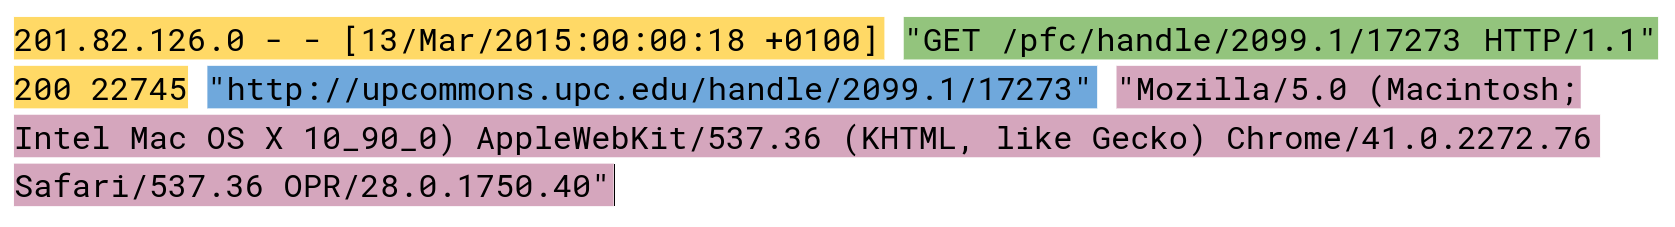
\includegraphics[width=\textwidth]{figures/example-log}\label{fig:log-example}
\end{figure}

\begin{itemize}[<+- | alert@+>]
    \item Informació de la petició HTTP.
    \begin{itemize}[<+- | alert@+>]
        \item Adreça IP
        \item Data i hora
        \item Informació de la petició HTTP
        \item Referent
        \item User Agent
    \end{itemize}
\end{itemize}

\end{frame}


\begin{frame}{Filtratge dels \textit{logs}}
    \begin{itemize}[<+- | alert@+>]
        \item Durant el processament hem trobat diverses casuístiques que s'han de tractar detalladament.
        \begin{itemize}[<+- | alert@+>]
            \item Accés a recursos web.
            \item Repeticions.
            \item Cerques.
            \item Errors de processament.
            \begin{itemize}[<+- | alert@+>]
                \item Errors reversibles.
                \item Errors irreversibles.
            \end{itemize}
        \end{itemize}
    \end{itemize}
\end{frame}


\begin{frame}{Disseny del processament dels logs}

    \begin{figure}
        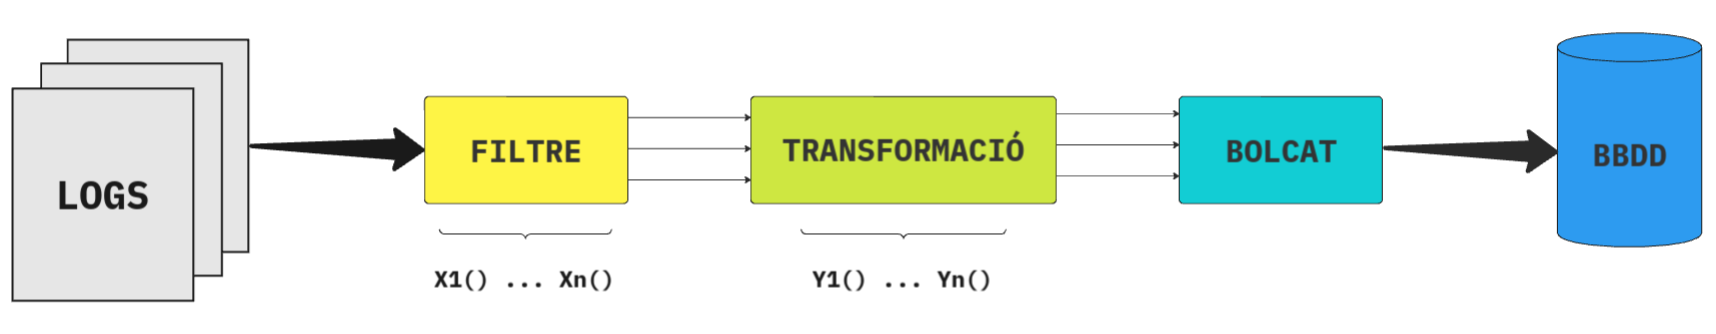
\includegraphics[width=\textwidth]{figures/log-processing}\label{fig:log-processing}
    \end{figure}

    \begin{itemize}[<+- | alert@+>]
        \item Tres components.
        \begin{itemize}[<+- | alert@+>]
            \item \texttt{Filtre} \(\rightarrow\) Filtra cada \textit{log} mitjançant un criteri específic.
            \item \texttt{Transformació} \(\rightarrow\) Modifica el format del \textit{log} per afegir o treure camps.
            \item \texttt{Bolcat} \(\rightarrow\) Adapta el format i envia el \textit{log} a la base de dades.
        \end{itemize}
    \end{itemize}
\end{frame}


\begin{frame}{Implementació del processament}
    \begin{figure}
        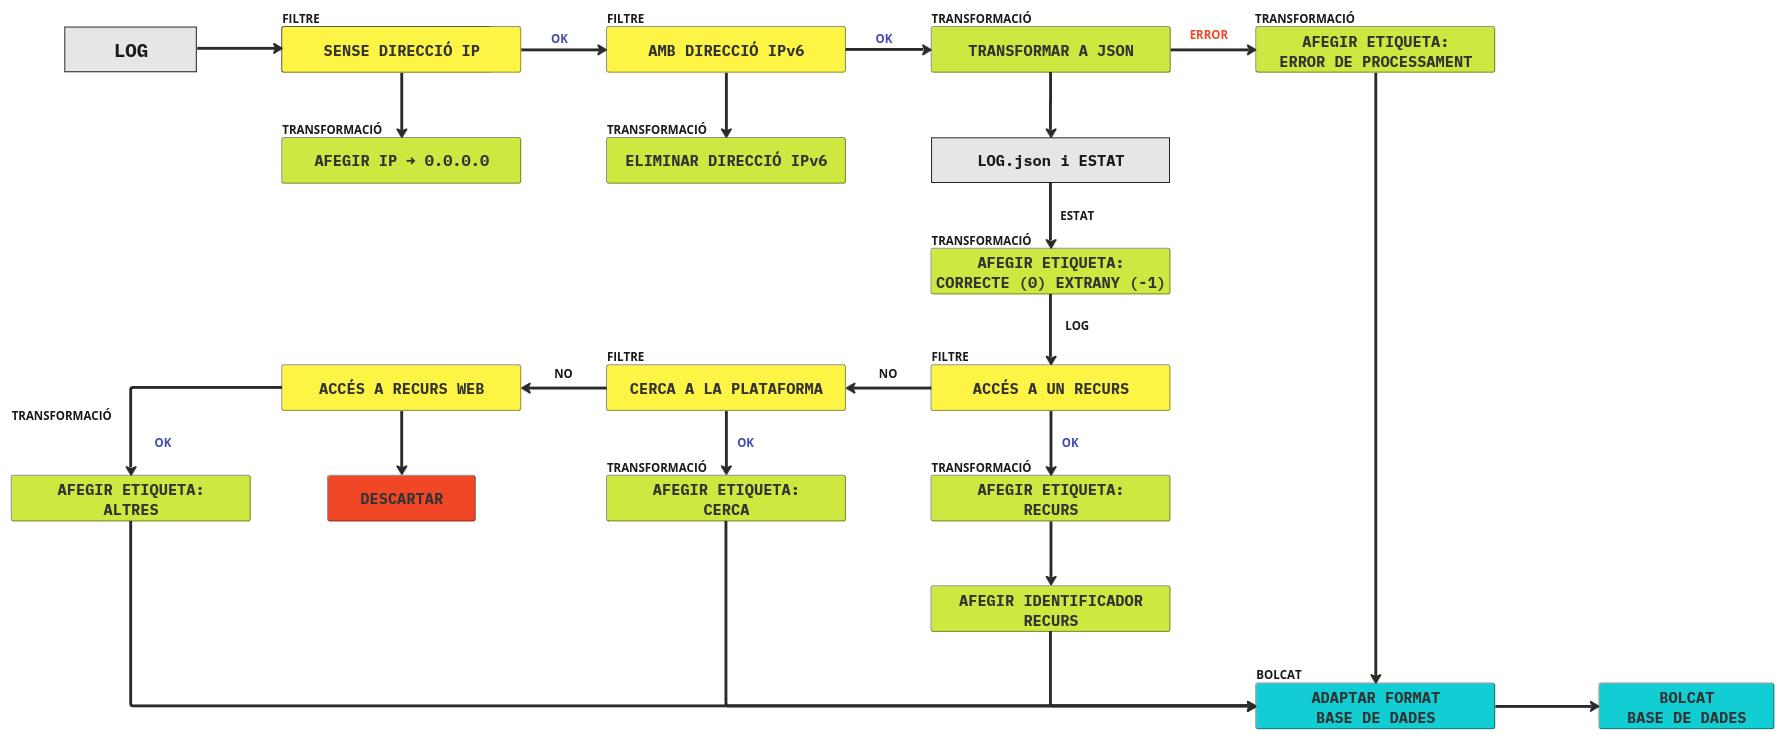
\includegraphics[width=1\textwidth]{figures/log-processing-workflow}\label{fig:log-processing-workflow}
    \end{figure}
\end{frame}


\begin{frame}{Metadades}
    \begin{itemize}[<+- | alert@+>]
        \item Conjunt d’etiquetes presents als recursos d’UPCommons que contenen informació sobre aquest.
        \item Format: DSpace Intermediate Metadata (DIM):
        \begin{itemize}[<+- | alert@+>]
            \item Dublin Core + qualificador.
        \end{itemize}
        \item Exemple: autor principal d'un recurs
        \begin{itemize}[<+- | alert@+>]
            \item \texttt{schema.element.qualifier} \(\rightarrow\) \texttt{dc.contributor.author}
        \end{itemize}
    \end{itemize}
\end{frame}